% Clue Selection Under Noise
%
% Build:  tectonic docs/clue-selection-theory.tex
% Output: docs/clue-selection-theory.pdf
%
% Tectonic downloads whatever packages this file needs on the first build
% and caches them, so there is no TeX distribution to install or maintain.

\documentclass[12pt]{article}

\usepackage[a4paper,margin=3.2cm]{geometry}
\usepackage{amsmath}
\usepackage{amssymb}
\usepackage{booktabs}
\usepackage{caption}
\usepackage{float}          % [H] pins the table and figure where they are written
% Blank line between paragraphs instead of a first-line indent. parskip
% also fixes up the spacing it would otherwise break around lists and
% display math, which setting \parindent and \parskip by hand does not.
\usepackage[skip=8pt, indent=0pt]{parskip}
\usepackage{microtype}
\usepackage[T1]{fontenc}
\usepackage{libertinus}          % swap for \usepackage{lmodern} to fall back
\usepackage{pgfplots}
\pgfplotsset{compat=1.18}

% arg max with the limits set underneath, as in the display.
\DeclareMathOperator*{\argmax}{arg\,max}

% Digits line up in columns in the results table.
\usepackage{siunitx}
\sisetup{table-number-alignment=right}

\begin{document}

% Title block by hand: \maketitle leaves a gap where the empty author
% would go, and the subtitle belongs directly under the title.
\begin{center}
  {\LARGE Clue Selection Under Noise}\\[0.7em]
  Codenames spymaster, baseline model
\end{center}
\vspace{1.5em}

\section{Introduction}
\label{sec:intro}

A clue is a clue word together with a number $k$. Whenever we give one, our
teammate ranks the unrevealed board words by how well each fits the clue word,
and chooses words from the top, stopping when they reach $k$ words or when
they choose a word that is not ours, whichever comes first.

Suppose we and our teammate order words by cosine similarities from the same
embedding space. Then choosing the optimal clue is just a search over the clue
vocabulary for the word with the longest starting run of our team's words in
the list sorted by decreasing similarity. In this case, our teammate chooses
only the words that we intend, and never chooses a word that is not ours. The
search is a matter of enumerating the vocabulary, and its solution is usually
not unique.

However, in practice, our perceived similarities are related to but different
from our teammate's, which changes the algorithm by which we find the optimal
clue. The problem becomes probabilistic rather than deterministic, and we now
have to account for the possibility of our teammate choosing a neutral,
opponent, or assassin word. This paper describes one algorithm for finding an
optimal clue under these conditions. 

\section{Setup}
\label{sec:setup}

Let $A$ be the set of our team's board words and $B$ the set of all other board
words. For any fixed clue word, let $z_x$ be its similarity to board word $x$,
standardized per clue word so that its similarities across the full board
vocabulary have mean $0$ and variance $1$.
Throughout this paper, $i$ indexes $A$ and $w$ indexes $B$.

In order to construct an algorithm, we first define rewards --- suppose
selecting a word of $A$ is worth $1$, and selecting $w \in B$ costs $c_w > 0$.
We want to choose the clue word and number $k$, with $1 \le k \le K$ for a
fixed maximum $K$, that maximizes the expected reward.

To model deviations in the guesser's perceived similarities of the words from
ours, we assume the guesser perceives board word $x$'s similarity with the clue
word as $\hat z_x = z_x + \varepsilon_x$, where the $\varepsilon_x$ are
independent $\mathcal N(0, \sigma^2)$ for some free parameter $\sigma$. We also
assume the guesser selects unrevealed words in decreasing order of $\hat z$,
stopping after $k$ selections or upon selecting a word of $B$, whichever comes
first.

Let
\[ T = \max_{w \in B} \hat z_w, \qquad W = \argmax_{w \in B} \hat z_w,
   \qquad N = \#\{\, i \in A : \hat z_i > T \,\}. \]
In words, $W$ is the non-team word with the highest similarity from the guesser, $T$ is the guesser's similarity of that word, and $N$ is the number of team words that the guesser ranks higher than $W$.

We know the guesser reveals
$\min(k, N)$ words of $A$, and selects a word of $B$ (that word being 
$W$) if and only if $N < k$. Note that no word of $B$ other than $W$ can be selected. Thus, our goal is to maximize $G(k) - P(k)$, where 
\[ G(k) = \mathbb E\bigl[\min(k, N)\bigr], \qquad
   P(k) = \mathbb E\bigl[\, c_{W}\,\mathbf 1\{N < k\} \,\bigr]. \]

\section{Derivation}
\label{sec:derivation}

Neither $G$ nor $P$ has a closed form. Both are expectations over all
$|A| + |B|$ noise variables at once, and the maximum of non-identical normals
has no elementary distribution, so the aim is not to solve them exactly but to
reduce them far enough to evaluate cheaply.

Our goal is to reduce both expressions to elementary operations and functions of $z_x$, the standard normal PDF and CDF, and single integrals.

We start with $G(k)$. Since $\min(k, N) = \sum_{j=1}^{k} \mathbf 1\{N \ge j\}$,
taking expectations and conditioning on $T$ gives
\[ G(k) \;=\; \sum_{j=1}^{k} \int \Pr(N \ge j \mid T = t) \,\, dF_T(t). \]
To evaluate this, we need the distribution of $T$ and the
distribution of $N$ given $T = t$.

For the first, let $\varphi$ and $\Phi$ be the PDF and CDF of a standard
normal, so that the PDF and CDF of $\hat z_w \sim \mathcal N(z_w, \sigma^2)$
are
\[ f_{\hat z_w}(t) = \sigma^{-1}\varphi\!\left(\frac{t - z_w}{\sigma}\right), \qquad
   F_{\hat z_w}(t) = \Phi\!\left(\frac{t - z_w}{\sigma}\right). \]
Since $T$ is a maximum of independent variables,
\[ F_T(t) \;=\; \prod_{w \in B} F_{\hat z_w}(t)
   \;=\; \prod_{w \in B} \Phi\!\left(\frac{t - z_w}{\sigma}\right). \]

For the second, note that $T$ is a function of $(\varepsilon_w)_{w \in B}$
only, which is independent of $(\varepsilon_i)_{i \in A}$. Thus conditioning on
$T = t$ does not change the distribution of the $\hat z_i$, and each $i \in A$
independently satisfies $\hat z_i > t$ with probability
\[ p_i(t) \;=\; \Phi\!\left(\frac{z_i - t}{\sigma}\right). \]
Thus, given $T = t$, $N$ is a sum of $|A|$ independent Bernoulli
variables, the $i$-th with success probability $p_i(t)$.

Now we move on to $P(k)$. Note that if we fix $T = t$, then $N$ is solely a function of $(\varepsilon_i)_{i \in A}$, whereas $W$ is solely a
function of $(\varepsilon_w)_{w \in B}$. Thus, $c_W$ and $\mathbf 1\{N < k\}$ are conditionally independent given $T$, so
\[ P(k) \;=\; \int \Pr(N < k \mid T = t)\; \bar c(t) \,\, dF_T(t), \qquad
   \bar c(t) = \mathbb E\bigl[\, c_{W} \mid T = t \,\bigr]. \]
We have already derived the distribution of $T$ and the first factor, so we just need $\bar c(t)$, which requires
$\Pr(W = w \mid T = t)$.

Writing $g_w$ for the joint density of $W = w$ and $T$ at $t$,
\[ \Pr(W = w \mid T = t) \;=\; \frac{g_w(t)}{f_T(t)}. \]
$W = w$ and $T = t$ means $\hat z_w = t$ and $\hat z_v < t$ for every
other $v \in B$. The $\hat z$ are independent, so
\[ g_w(t) \;=\; f_{\hat z_w}(t) \prod_{v \ne w} F_{\hat z_v}(t). \]
The events $\{W = w\}$, $w \in B$, are disjoint and exhaustive, so
\[ f_T(t) \;=\; \sum_{w \in B} g_w(t). \]
Since $F_T(t) = \prod_{v \in B} F_{\hat z_v}(t)$, the product over $v \ne w$ is
$F_T(t) \big/ F_{\hat z_w}(t)$. Set
\[ h_w(t) \;=\; \frac{f_{\hat z_w}(t)}{F_{\hat z_w}(t)}
   \;=\; \frac{\sigma^{-1}\varphi\bigl((t - z_w)/\sigma\bigr)}
              {\Phi\bigl((t - z_w)/\sigma\bigr)}, \]
so that $g_w(t) = F_T(t)\, h_w(t)$ and $f_T(t) = F_T(t) \sum_v h_v(t)$. The
$F_T(t)$ cancels in the ratio:
\[ \Pr(W = w \mid T = t) \;=\; \frac{h_w(t)}{\sum_v h_v(t)}, \qquad
   \bar c(t) \;=\; \frac{\sum_w c_w\, h_w(t)}{\sum_w h_w(t)}. \]

\section{Numerical evaluation}
\label{sec:computation}

Both $G$ and $P$ have the form $\int \psi(t)\, dF_T(t)$ for a bounded $\psi$:
\[ \psi_G(t) = \sum_{j=1}^{k} \Pr(N \ge j \mid T = t), \qquad
   \psi_P(t) = \Pr(N < k \mid T = t)\, \bar c(t). \]
Both are evaluated by numerical integration. Partition an interval
$[t_0, t_M]$ into cells $[t_m, t_{m+1}]$, take $\psi$ at the midpoint
$\bar t_m = \tfrac{1}{2}(t_m + t_{m+1})$ of each, and weight it by the
probability that $T$ lands in that cell:
\[ u_m \;=\; F_T(t_{m+1}) - F_T(t_m), \qquad
   \int \psi(t) \, dF_T(t) \;\approx\; \sum_m \psi(\bar t_m)\, u_m. \]
Because the range of $T$ is $\mathbb{R}$, we have to limit our integral approximation to bounds $t_0$ and $t_M$. Take $t_0$ below every $z_w$ and $t_M$ above every $z_w$, each by several
$\sigma$, so that $F_T(t_0)$ and $1 - F_T(t_M)$ are negligible. 

Computing $\bar c(t)$ takes $O(|B|)$. 

The probabilities $\Pr(N \ge j \mid T = t)$ follow from
the standard recursion for a sum of independent Bernoulli variables. Letting
$q^{(i)}_r$ be $\Pr(N = r)$ after the first $i$ words of $A$,
\[ q^{(0)}_0 = 1, \qquad
   q^{(i)}_r \;=\; q^{(i-1)}_r\bigl(1 - p_i(t)\bigr)
                \;+\; q^{(i-1)}_{r-1}\,p_i(t), \]
and $\Pr(N \ge j \mid T = t) = 1 - \sum_{r < j} q_r$. Counts above $K$
are never used, so this takes $O(|A|K)$.

The total is $O\bigl(M(|A|K + |B|)\bigr)$ per clue, with $M$ the number of
cells. 

\section{Results}
\label{sec:results}

The model has one free parameter. To choose it, $\sigma$ was swept and each
setting was made to play full two-team games against a fixed opponent, the
centroid baseline, over 100 games per setting. Every board is played twice with
the sides swapped, because team $A$ holds nine words and moves first while team
$B$ holds eight, so a one-sided run would confound the parameter with that
advantage. The guesser on both sides was Claude Sonnet, prompted to rank the
unrevealed board words by how related each is to the clue word. Turns are scored
as the game scores them: $+1$ per word of $A$ revealed, and $-0.2$, $-1$ and
$-10$ for a neutral, opponent and assassin word.

\begin{table}[H]
\centering
\small
\begin{tabular}{
  S[table-format=1.2] S[table-format=2.0]
  S[table-format=1.2] S[table-format=1.2] S[table-format=1.2] S[table-format=1.2]
  S[table-format=2.0]}
\toprule
{$\sigma$} & {win \%} & {announced $k$} & {own/turn} & {advantage/turn}
  & {reward/turn} & {assassin \%} \\
\midrule
 1.0  & 69 & 2.67 & 1.48 & 1.24 & 0.85 & 14 \\
 1.25 & 70 & 2.27 & 1.43 & 1.23 & 1.01 &  8 \\
 1.5  & 70 & 1.93 & 1.33 & 1.17 & 1.01 &  6 \\
 2.0  & 57 & 1.42 & 1.17 & 1.10 & 1.05 &  2 \\
 2.5  & 51 & 1.16 & 1.07 & 1.04 & 0.98 &  3 \\
\bottomrule
\end{tabular}
\caption*{\footnotesize Per turn, over 100 games per setting.
\emph{announced} is $k$; \emph{own/turn} is how many words of $A$ the guesser
actually took; \emph{advantage} subtracts the opponent words it gave away;
\emph{assassin} is the share of games lost outright.}
\end{table}

\begin{figure}[H]
\centering
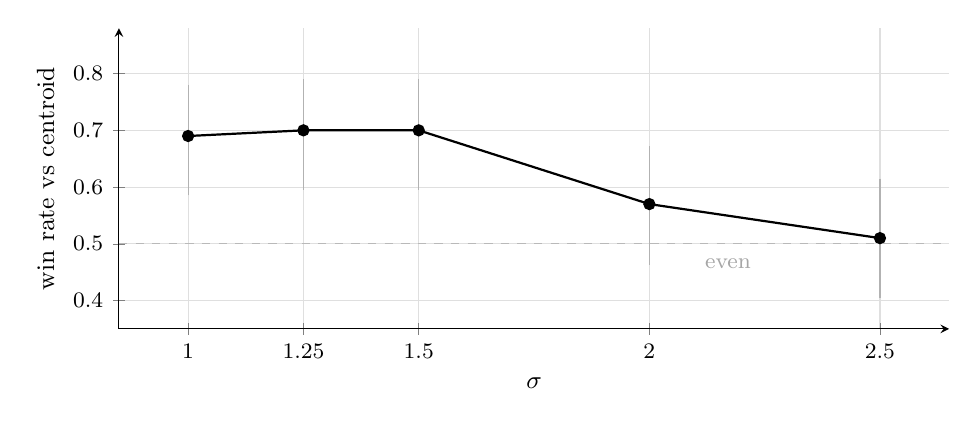
\begin{tikzpicture}
\begin{axis}[
  width=\linewidth, height=5.4cm,
  xlabel={$\sigma$}, ylabel={win rate vs centroid},
  xmin=0.85, xmax=2.65, ymin=0.35, ymax=0.88,
  xtick={1.0,1.25,1.5,2.0,2.5},
  ytick={0.4,0.5,0.6,0.7,0.8},
  grid=major, grid style={gray!25, thin},
  axis lines=left,
  tick label style={font=\footnotesize}, label style={font=\small},
  every axis plot/.append style={thick},
]
\addplot+[
  mark=*, mark size=1.8pt, black, mark options={fill=black, draw=black},
  error bars/.cd, y dir=both, y explicit,
  error bar style={gray!60, thin}, error mark options={gray!60},
] table[x=sigma, y=win, y error minus=lo, y error plus=hi] {
sigma win   lo    hi
1.0    0.69 0.096 0.082
1.25  0.70 0.096 0.081
1.5   0.70 0.096 0.081
2.0   0.57 0.098 0.093
2.5   0.51 0.097 0.096
};
\draw[gray!55, dashed] (axis cs:0.85,0.5) -- (axis cs:2.65,0.5);
\node[anchor=west, font=\footnotesize, gray!70] at (axis cs:2.1,0.465) {even};
\end{axis}
\end{tikzpicture}
\caption*{\footnotesize Win rate against the centroid baseline, 100 games per
setting. Bars are 95\% Wilson intervals. The plateau from $1.0$ to $1.5$ is flat
within noise; $2.0$ and $2.5$ are clearly below it, and $2.5$ is
indistinguishable from an even match.}
\end{figure}

\begin{figure}[H]
\centering
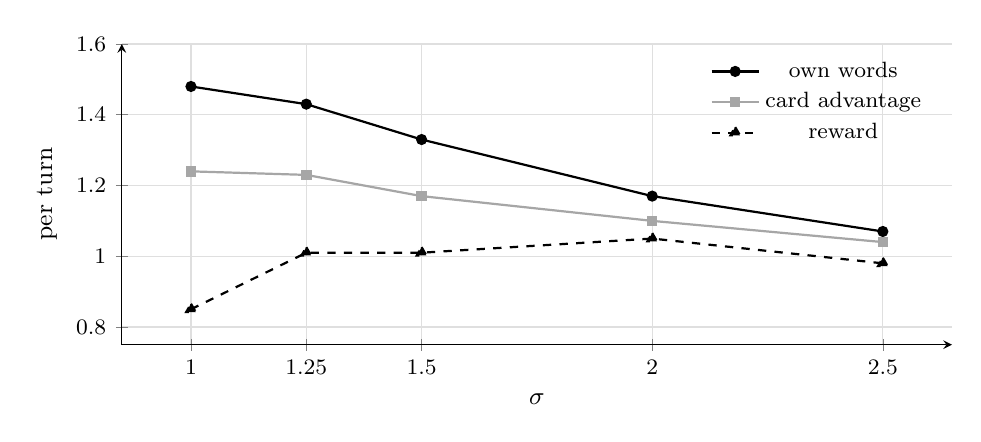
\begin{tikzpicture}
\begin{axis}[
  width=\linewidth, height=5.4cm,
  xlabel={$\sigma$}, ylabel={per turn},
  xmin=0.85, xmax=2.65, ymin=0.75, ymax=1.6,
  xtick={1.0,1.25,1.5,2.0,2.5},
  grid=major, grid style={gray!25, thin},
  axis lines=left,
  legend style={at={(0.98,0.98)}, anchor=north east, font=\footnotesize,
                draw=none, fill=none},
  tick label style={font=\footnotesize}, label style={font=\small},
  every axis plot/.append style={thick},
]
\addplot[mark=*, mark size=1.6pt, black] coordinates
  {(1.0,1.48) (1.25,1.43) (1.5,1.33) (2.0,1.17) (2.5,1.07)};
\addlegendentry{own words}
\addplot[mark=square*, mark size=1.5pt, gray!70] coordinates
  {(1.0,1.24) (1.25,1.23) (1.5,1.17) (2.0,1.10) (2.5,1.04)};
\addlegendentry{card advantage}
\addplot[mark=triangle*, mark size=2pt, black, dashed] coordinates
  {(1.0,0.85) (1.25,1.01) (1.5,1.01) (2.0,1.05) (2.5,0.98)};
\addlegendentry{reward}
\end{axis}
\end{tikzpicture}
\caption*{\footnotesize The three per-turn measures. Words taken falls
monotonically with $\sigma$; reward does not vary.}
\end{figure}

Win rate is flat from $\sigma = 1.0$ to $1.5$ and falls away above it. Words
taken per turn falls monotonically across the whole range, while reward per
turn does not vary: every setting from $1.25$ upward lies between $0.98$ and
$1.05$, so it does not distinguish them.

We take $\sigma = 1.5$ from here on --- the top of the win-rate plateau, at its
cautious end, since $1.0$ and $1.25$ win no more often while ending turns on
the assassin more than twice as frequently.

\end{document}
